\chapter{GEOMETRY}
% !TEX root = hazy1.tex

\section{Overview}

This section describes commands that determine the geometry of the
emission-line region.
Many of the quantities used below are defined in
the section on geometry in the Chapter \cdSectionTitle{DEFINITIONS}.

The geometry is always spherical but can be made effectively plane
parallel by making the radius much greater than the
thickness of the nebula.
It is also possible to compute a model in which the emission-line region
is almost a disk.
A covering or filling factor can be specified and the
cloud can be either static or expanding.

\section{Age 44 years [off]}

For an equilibrium geometry the code assumes that the cloud is old enough for
atomic processes to have become time steady.
The \cdCommand{age} command allows the
code to confirm that the microphysics is indeed time steady.
The age of
the cloud is given on the command line.
The default units are linear
seconds.
The keyword \cdCommand{log} will force the code to interpret the number as
a log.
The keywords \cdCommand{minutes}, \cdCommand{days}, \cdCommand{weeks},
\cdCommand{fortnights}, \cdCommand{months}, \cdCommand{years},
\cdCommand{centuries}, and \cdCommand{millennia} change the units.

The code keeps track of many timescales during a calculation.
After the calculation is complete it will check that none of the
equilibrium timescales for significant physical processes
were longer than the age of the cloud.
The code will complain if the age of the cloud is not set but
still compute the model.
If a physical process is not significant, for
instance, the \htwo\ formation timescale in a highly-ionized gas,
the age is
set to a negative number.
This retains the value while not including the
process as a significant part of the physical simulation.

If the keyword \cdCommand{off} appears then the age will not be checked.

\section{Aperture commands}

\subsection{Aperture [slit, beam]}

The \cdCommand{aperture} command simulates observing
a part of the computed structure
with a spectrometer.
It was first incorporated into the code by Peter van
Hoof who wrote the original version of this section.

One of the keywords \cdCommand{slit} or \cdCommand{beam} must appear.
The keyword \cdCommand{beam} tells
the code to simulate observing a resolved nebula with a
small pencil beam centered very close to the central source.
If the keyword \cdCommand{slit} appears then the computed structure
is simulated to be observed with a long slit that extends
over the {\em entire} width of the nebula, also positioned
very close to the center. In the long slit case, it is assumed
that the observer has added up all the flux from the source over the
full length of the slit. It is not now possible to simulate
an off-axis long slit or pencil beam.

The \cdCommand{aperture} command only affects how volume
emissivities are added
together to form the final line spectrum printed in the main \Cloudy\
output and saved with the \cdCommand{save lines} command.
When optimizing line fluxes, or line flux ratios, the quantities
observed through the aperture will be used.
This command has no effect on any aspect of
the calculation of conditions in the gas.
It also does {\em not} affect the spectral energy distribution
predicted with the \cdCommand{save continuum} commands.
This will always be integrated over the entire nebula.
The continuum bands in the file \cdFilename{data/continuum\_bands.ini} are not
predicted when the \cdCommand{aperture} command is used, for this reason.

This command only affects the line luminosities in the luminosity case.
When the intensity case is used and the inner radius
is not specified all integrations are for a pencil beam through a plane-parallel slab.

In the following a quantity $\alpha$ is defined
with the following meaning:
$\alpha = 0$ in the pencil beam case
(we are observing along a single line of sight
passing through the center of the nebula),
$\alpha = 1$ in the long-slit case (we
are observing through a narrow slit placed over the center of the nebula;
the slit is longer than the nebula and the
flux is integrated over the entire
slit), and $\alpha = 2$ in the general case
(we are observing the flux integrated
over the entire nebula).
The default index is $\alpha = 2$.

In all cases an observed quantity $Q_{\alpha }$ can be defined for a
line $\lambda $ as
\begin{equation}
Q_\alpha  \left( \lambda  \right) = C_\alpha  D_\alpha  \int {\left(
{\frac{r}{{r_0 }}} \right)^\alpha  } \varepsilon \left( \lambda  \right)dr
,% (39)
\end{equation}
where $\varepsilon (\lambda )$ is the line's volume emissivity [erg
cm$^{-3} \mathrm{s}^{-1}$] and
\begin{equation}
\begin{array}{ll}
 C_0&  = 2 \\
 C_1&  = 2\pi r_{\mathrm{0}}  \\
 C_2&  = 4\pi r_{\mathrm{0}}^{\mathrm{2}}  \\
 \end{array},% (40)
\end{equation}
where $r_{\mathrm{0}}$ is the inner radius of the nebula.  The covering factor
$D_\alpha $ depends
on the geometry and is
\begin{equation}
\label{aper_cover}
\begin{array}{ll}
 D_0&  = 1/2,\;\;1 \\
 D_1&  = \Theta /2\pi  \\
 D_2&  = \Omega /4\pi  \\
 \end{array}
.% (41)
\end{equation}
For the entire nebula $(\alpha  = 2)$ this is the familiar definition
(see also Sect.~\ref{cov_factor}).
In the long
slit case ($\alpha  = 1$), $D_1$ is the fraction of a large circle in the plane that
is being observed that actually passes through nebular material.
In the pencil
beam case ($\alpha  = 0$), $D_0$ indicates whether only the front or back side of the
line of sight is covered with nebular material ($D_0 = 1/2$)
or if both sides
are covered ($D_0 = 1$).
The covering factor for the entire nebula is set
with the \cdCommand{covering factor} command. This is the quantity $D_2$.
You can set the quantities $D_0$ or $D_1$ using the \cdCommand{aperture covering factor}
command described below.

In the luminosity case $Q_\alpha $ will have units erg s$^{-1}$
for the entire nebula,
erg cm$^{-1}$ s$^{-1}$ for the long slit case,
and erg cm$^{-2}$ s$^{-1}$ for the pencil beam.
In the intensity case the units are erg cm$^{-2}$ s$^{-1}$.
The luminosity and intensity cases
are defined on page \pageref{sec:IntensityLuminosityCases}.

$Q_\alpha$ is the quantity printed in the main \Cloudy\ output and by the
\cdCommand{save lines} command in the default setup. However, if the
distance to the object is set with the \cdCommand{distance} command,
we can convert this quantity into an observed flux at Earth.
In the luminosity case we can construct the following relations between observed
quantities and the quantities predicted by the code.  These neglect
interstellar extinction of course.
The flux measured at the Earth will be
\begin{equation}
F_\alpha  \left( \lambda  \right) = \frac{{A_\alpha  }}{{4\pi D^2
}}\;Q_\alpha  \left( \lambda  \right)\, [\mathrm{erg\, cm}^{-2} \mathrm{s}^{-1}],% (42)
\label{flux_conversion}
\end{equation}
with
\begin{equation}
\label{flux_conv_aperfac}
\begin{array}{ll}
 A_0&  = \Omega _b D^2  \\
 A_1&  = \Theta _s D \\
 A_2&  = 1 \\
 \end{array}
.% (43)
\end{equation}
Here $F_\alpha $ is the observed flux
[erg cm$^{-2}$ s$^{-1}$]
$D$ is the distance of the object [cm],
as specified with the \cdCommand{distance} command,
$\Theta_s$ is the slit width [radian],
and $\Omega_b$ is the surface area of the pencil beam [sr].

If the \cdCommand{print line flux at Earth} command is used, then \Cloudy\ will
do this conversion for you and $F_\alpha$ will be reported in the main \Cloudy\
output as well as the \cdCommand{save lines} output. $F_\alpha$ will then also be
used when optimizing line fluxes. You can set the value of $\Theta_s$ or $\Omega_b$
with the \cdCommand{aperture size} command described below.

In the intensity case (the intensity case implies $\alpha  = 0$)
the relation
between the observed surface brightness
$S(\lambda )$ and $Q_o(\lambda )$ is simply:
\begin{equation}
S\left( \lambda  \right) = \frac{{\Omega \left( {1\;{\mathrm{arcsec}}^2 }
\right)}}{{4\pi }}\;Q_0 \left( \lambda  \right) \approx 1.87043 \times 10^{
- 12} Q_0 \left( \lambda  \right)
\, [\mathrm{erg\, cm}^{-2}\; \mathrm{s}^{-1}\; \mathrm{arcsec}^{-2}] .
\end{equation}

\subsection{Aperture size 2.5}

This command should be used in conjunction with the \cdCommand{aperture [slit,
    beam]} and \cdCommand{print line flux at Earth} commands. It will have no
effect otherwise. It allows you to set the slit width [arcsec] or the surface
area of the pencil beam [arcsec$^2$]. These are the quantities $\Theta_s$ and
$\Omega_b$ used in Eq.~\ref{flux_conv_aperfac}. The quantity entered will
always be treated as a linear quantity. If this command is not used, the code
will assume a default slit width of 1~arcsec, or a beam area of 1~arcsec$^2$.

\subsection{Aperture covering factor 0.6}

This command should be used in conjunction with the \cdCommand{aperture [slit,
    beam]} command. It allows you to set the quantity $D_\alpha$ defined in
Eq.~\ref{aper_cover}. A single number should appear on the command line
which should be between 0 and 1. The default value is 1.

\section{Clumping factor = 0.05 [index =-1]}
This is a another name for the
\cdCommand{filling factor} command described on
page \pageref{sec:CommandFillingFactor}.
It takes the same options, and includes the same physics,
as described there.

\section{Covering factor 0.3}
\label{cov_factor}

This sets a covering factor $\Omega/4\pi$ for the emission-line region
(see AGN3 section 5.9).
The argument is the log of the covering factor
if less than or equal to zero and the linear covering factor if positive.
It is impossible to specify a covering factor of zero.

The covering factor affects both the luminosity of the emitted spectrum
and the radiative transfer of lines and continua.
If a covering factor
is set and the luminosity case used then the luminosities
will be for a shell covering $\Omega$ sr of the central object.
Line luminosities
will scale nearly linearly with the covering factor.
The covering factor
does not strongly affect the line intensities in the intensity case, where
the emission per unit area of cloud is considered.
The covering factor
does have second-order effects on the spectrum because of changes in the
transport of the diffuse radiation fields.

This covering factor is referred to as the geometric covering factor,
and is stored as the variable \cdVariable{covgeo}.
A second covering factor,
\cdVariable{covrt},
affects the transfer of lines and continua.
This command sets both covering factors.

If no covering factor is entered and \cdCommand{sphere}
is not set (see section \ref{sec:CommandSphere}) then the default
is for a geometric covering factor of unity (the shell fully covers the
continuum source) but a radiative covering factor of zero (i.e., an open
geometry).

\section{Cylinder log semi height =9.12}

\noindent The model will be spherical,
but truncated so as to simulate a cylinder
(see \citealp{FerlandLambert1982}).
Figure \ref{fig:cylin} gives an example of the assumed geometry.

\begin{figure}
\centering
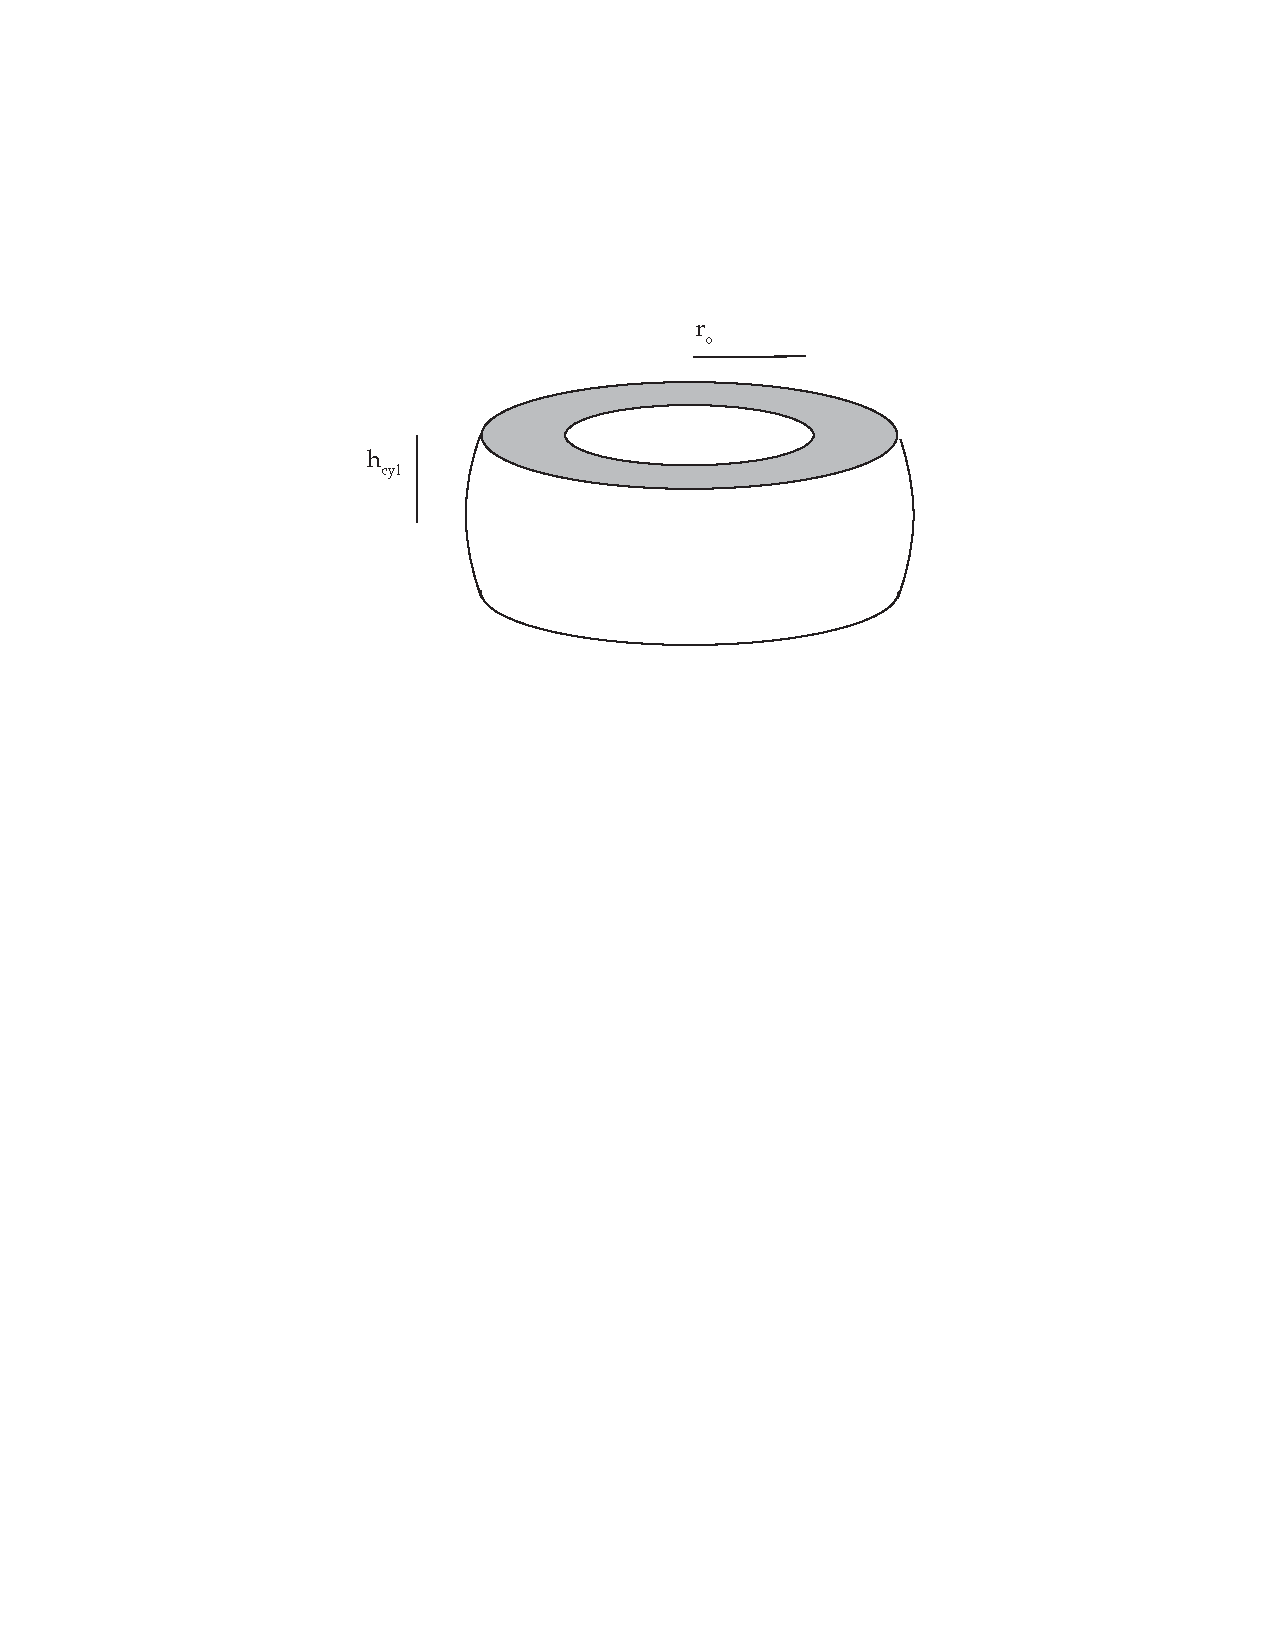
\includegraphics{cylin}
\caption[Cylindrical geometry]
{\label{fig:cylin}This figure shows the geometry assumed when the \cdCommand{cylinder} command
is used.}
\end{figure}

The inner and outer radii of the cylinder are set by
the \cdCommand{radius} command.
The \cdCommand{cylinder} command sets the full height of
the cylinder to twice the number entered on the command.
The argument is
the log of the semi-height in cm.

The effective volume element used to compute the emissivity of the gas
is given by
\begin{equation}
\label{eqn:cylin}
d{\kern 1pt} V = 4{\kern 1pt} \pi \,r_{\mathrm{o}}^2 \left( {\frac{r}{{r_{\mathrm{o}}
}}} \right)\left( {\frac{{\min \left( {r,\;h_{cyl} } \right)}}{{r_{\mathrm{o}}
}}} \right)\;f\left( r \right)\;dr
\,[\mathrm{cm}^{3}]% (45)
\end{equation}
where $r_{\mathrm{o}}$ is the inner radius, $h_{cyl}$ is the cylinder
half-height, and $f(r)$
is the filling factor.
The default value is $h_{cyl}= 10^{35}$~cm.

Changing the emissivity as described by equation \ref{eqn:cylin}
is the only effect of this command.
It does not alter the radiative transfer methods and is
only formally correct when the continua and lines are optically thin.

When combined with the \cdCommand{aperture slit} command, it will be assumed
that the slit is oriented along the rotational axis of the cylinder. If the
slit is oriented at an angle, you can model this geometry by dividing the
height of the cylinder by the cosine of the angle. If the slit is
perpendicular to the rotational axis you can simply omit the cylinder command
since it will have no effect on the predicted spectrum.

\section{Distance 3.2 linear parsecs}

This sets the distance to the object from the Earth.
The number is the
log of the distance in centimeters.
The \cdCommand{linear} keyword forces the number
to be interpreted as the linear distance and the
\cdCommand{parsecs} keyword changes
the units to parsecs.

If the distance is set then it is possible to predict the emission-line
fluxes observed at Earth if the luminosity case is
computed.
If the distance is set with this command then the observed
emission-line fluxes at the Earth will be printed if the
\cdCommand{print line flux}
command is also entered.

This command can be combined with the \cdCommand{aperture} command
to simulate observing parts of a nebula from the Earth.

\section{Filling factor = 0.05 [index =-1]}
\label{sec:CommandFillingFactor}

The first number is the filling factor $f(r)$ for a clumpy model (AGN3
Section 5.9).
It can be either the filling factor itself (which is greater
than zero and less than or equal to one) or the log of the filling factor
(if it is less than or equal to zero).
The second optional number is the
index  for a power-law variation of the filling factor $f(r)$, i.e.,
\begin{equation}
f\left( r \right) = f\left( {r_{\mathrm{o}} } \right)\left( {\frac{r}{{r_{\mathrm{o}}
}}} \right)^\alpha
%(46)
\end{equation}
where $r_{\mathrm{o}}$ is the inner radius of the cloud.

The filling factor is used in two ways.  The first is to modify the volume
emissivity of the gas,
\begin{equation}
dE = \varepsilon \,f\left( r \right)\,\,dV\,\frac{\Omega }{{4\,\pi }}
\,[\mathrm{erg\, s}^{-1}]% (47)
\end{equation}
where $\Omega/4\pi$ is the covering factor.
The second is to modify the optical depth scale
\begin{equation}
d\tau  = \alpha _{l,u} \left( {n_l  - n_u \frac{{g_l }}{{g_u }}}
\right)f\left( r \right)\,dr
%(48)
\end{equation}
(see \citealp{Osterbrock1959}).

A filling factor greater than unity is not allowed.  \Cloudy\ will set
a filling factor of unity if a value greater than one is entered.   The
code will complain (but compute the model) if a filling factor is set in
a constant pressure model since this makes no physical sense.

\section{Illumination angle 45 deg [radians]}

The plane-parallel slab is illuminated by a beam $\theta $
away from the normal.
The default is $\theta  = 0$ (normal illumination).
The angle is in degrees unless
the keyword \cdCommand{radian} appears.

The only effect of this command is to cause the beam of incident radiation
to be attenuated by $\tau n / \cos(\theta )$ where $\tau n$
is the normal optical depth of the zone.
The line and diffuse continua optical depth scale, which is
defined normal to the plane, are not directly affected by this command.

\emph{N.B.}  If this is used with the \cdCommand{grid} or
\cdCommand{vary} options the angle must be given in radians.
See the discussion of the commands with a \cdCommand{vary} option.

\section{Radius r(inner)  [r(outer), thickness; parsec; linear]}
\label{sec:RadiusCommand}

The first number is the log of the inner radius.
The second optional
number sets a stopping radius and is either the log of the
outer radius
(if it is larger than the first number) or the log of the thickness of the
cloud (if it is less than or equal to the first number).

The numbers are normally interpreted as the log of the radii in cm.
If the optional keyword \cdCommand{linear} appears then
the numbers are interpreted
as linear numbers.
The default units are centimeters.
The arguments will
be interpreted as the log of the radii in parsecs if the keyword
\cdCommand{parsec} appears.
Arguments will be interpreted as linear parsecs if both keywords
appear.
The following gives examples of its use.
\begin{verbatim}
radius 19.5       # log of inner radius in cm
radius 19.5 18.5  # as above, but a thickness of 3x10^18 cm
radius 19.5 20    # inner radius as above, outer radius 10^20 cm
radius 100 linear # inner radius of 100 cm
radius 0 parsecs  # log of radius in parses, so inner radius 1 pc
radius 1 to 3 linear parsecs # inner radius 1 pc, outer 3 pc
\end{verbatim}

The default outer radius is effectively infinite (actually $10^{31}$~cm).
If the intensity case is used then a starting radius of $10^{30}$~cm
will be set by default.
Under most circumstances this will result in a
plane-parallel geometry.

Page \pageref{sec:RadiusVaryOptions} describes a problem
that can occur if the second parameter is used with the
\cdCommand{vary} option.
Please read it if you will vary the radius
with the outer radius set.
The \cdCommand{stop thickness} command provides a way to set
a stopping thickness without specifying a starting radius.

\section{Sphere [options]}
\label{sec:CommandSphere}

\Cloudy\ normally assumes an open geometry, i.e.,
that the gas covering factor is small.
The \cdCommand{sphere} command\footnote{The \cdCommand{slit} and \cdCommand{beam}
options were recognized by the \cdCommand{sphere} command before
version 96.  These options were moved to the \cdCommand{aperture} command which was
introduced in version 96.} \footnote{Before version 96 the \cdCommand{sphere} command included an option to change
the covering factor.  The covering factor was removed from the
\cdCommand{sphere}
command.  Only the \cdCommand{covering factor} command changes the covering
factor.} should be included
to change this assumption for a closed geometry,
one where the covering factor of the gas is large and the model spherical.
This command tells \Cloudy\ to take into account ionization by the diffuse
continua and lines produced in the far side of the nebula
(i.e., from beyond the central object), and not to attenuate
the ionizing continuum by pure
scattering opacities, such as electron scattering,
back scattering by grains,
or Rayleigh scattering.

This option should be set when the geometry is spherical and gas nearly
fully covers the continuum source.
It should not be set when the covering
factor is small so that emission from a cloud is unlikely to encounter
another cloud.
This latter case is the default.
In the language of Van
Blerkom and Hummer (1967), \cdCommand{sphere}
causes \Cloudy\ to assume the symmetric
case (their equation 2.14),
rather than the default zero case (their equation
2.13) for diffuse continua.
Here these are referred to as closed and open
geometries, respectively.

Situations can occur where it is not obvious whether or not
\cdCommand{sphere} should
be used.
In this case it would be best to compute models with and without
\cdCommand{sphere} and compare results.
In most cases this will only make a 10--15\%
difference in predicted quantities.

\subsection{Sphere expanding or static}

Two optional keywords,
\cdCommand{expanding} and \cdCommand{static},
determine how line transfer
is handled.
If \cdCommand{expanding} (the default when
\cdCommand{sphere} is entered) is set then
\Cloudy\ assumes that line photons escaping
from the illuminated face of the
cloud are Doppler shifted away from lines of
absorbing material on the far
side of the shell.
This will be the case if the expansion velocity exceeds
the Doppler width by large amounts.
If \cdCommand{static} is set then line photons
do interact on both sides so that even line photons produced at the
illuminated face of the cloud will be strongly trapped by material on the
far side.
$L\alpha $ radiation pressure in the \hplus\ region will probably be
significant if \cdCommand{sphere static} is set and grains are not present.

It is necessary to iterate at least one time when
the \cdCommand{static} option is
used since the total line optical depths are not known on the first
iteration.
All optical depths are determined self-consistently on second
and further iterations.

The specific effects of \cdCommand{sphere} are the following:
The total continuous
optical depths are assumed to be twice the computed optical depths, and
the initial optical depth is half the total.
All diffuse reemission
(bremsstrahlung, free-bound, etc.) is counted in the outward beam
rather than only half.
Scattering opacities are not considered in the attenuation
of the incident radiation field.
When \cdCommand{static} is set, the optical depth
in L$\alpha$ in the inner direction is set to 10$^5$ on the first iteration.
Otherwise it is 10$^{-20}$.
The total optical depths of lines are twice their computed
depth for the static case.
Finally, ionization by lines and continua
produced in the far side of the nebula is included.
At the end of the
iteration all inward optical depths are set to half of the total value
computed from the previous iteration.

\section{Stop depth\dots}

\section{Stop thickness\dots}

The \cdCommand{stop depth} and \cdCommand{stop thickness} commands
provide methods to set the thickness of a cloud without
specifying its radius.
They are described in other sections.






